\section{Architecture}
In the following, we describe the architecture of \textit{helios}, which is currently designed as shown in Figure~\ref{fig:hardarchitecture}:
\textit{helios} acts as an intermediary layer between the game as a real-time data model~\cite[525]{Gre19} and the technical infrastructure.
The framework visualizes the game state and transmits input data to the game as control commands.

\begin{figure}[!h]
    \centering
    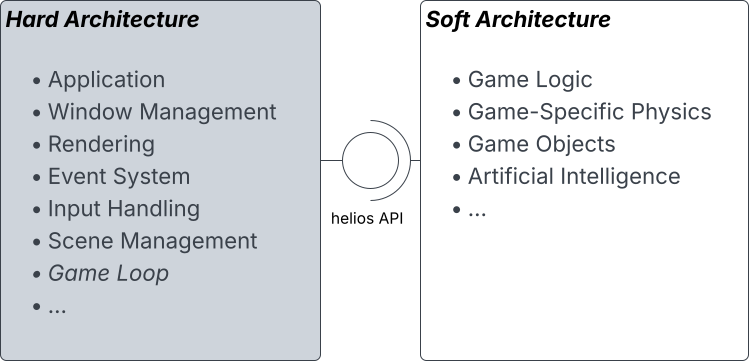
\includegraphics[width=0.8\columnwidth]{img/hardarchitecture_en.svg}
    \caption{Division of the architecture of the \textit{helios} framework into \textit{hard} and \textit{soft architecture} according to Rollings and Morris~\cite[612]{RM04}.
    The ball-and-socket notation illustrates that \textit{helios} provides interfaces that can be used by any game. (Source: own representation)}
    \label{fig:hardarchitecture}
\end{figure}

Figure~\ref{fig:package_diagram} shows a more detailed view of the modules and selected components.
The directory structure of \textit{helios} mirrors the structure of its core functionalities.
In the sense of \textit{Evans}, this is crucial for high cohesion: the directory names communicate the functionalities they contain~\cite[pp.~180-181]{Eva03}.
Within the modules, there is a further subdivision into layers (such as \texttt{controller}), following a ``package-by-feature and -by-layer`` design approach.

\begin{figure*}[t]
    \centering
    \makebox[\textwidth][c]{%
        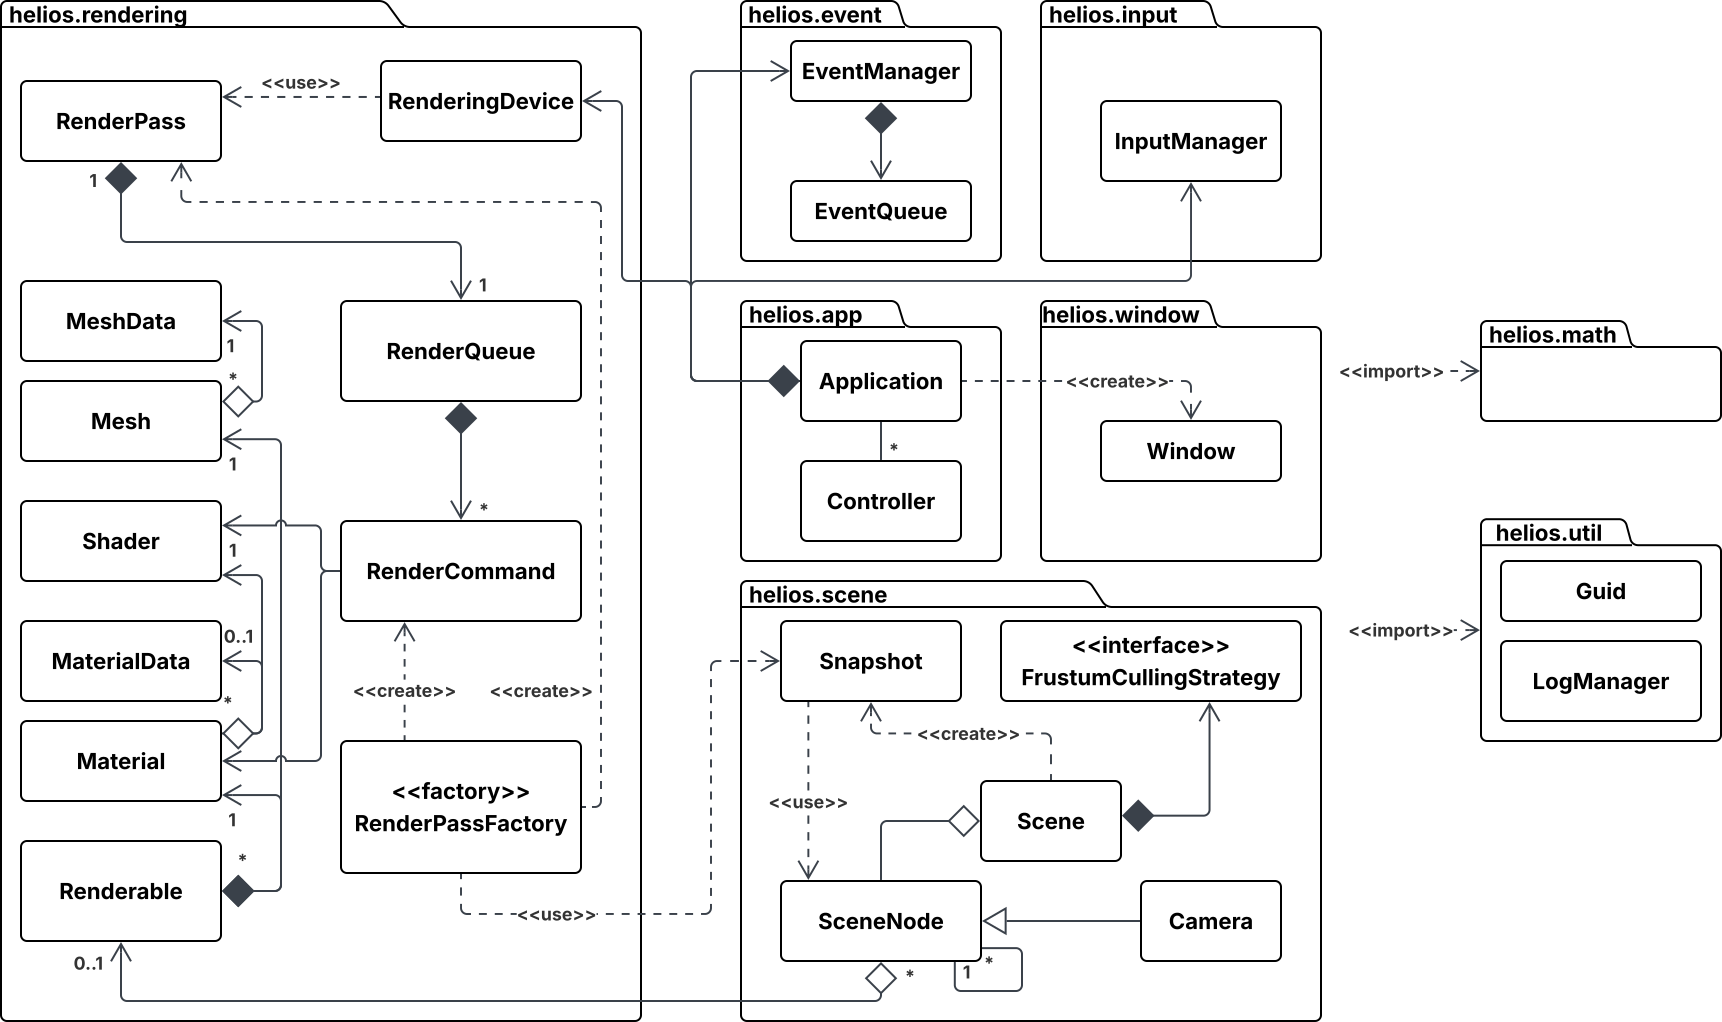
\includegraphics[width=1\textwidth]{img/package_diagram.svg}
    }
    \caption{Structure of the \textit{helios} framework and relationships between selected components.
    The modules follow a ``by-feature, by-layer`` concept in which features are internally divided into functional layers. (Source: own representation)}
    \label{fig:package_diagram}
\end{figure*}

\subsection*{\texttt{app}: Application layer}

The central control unit of the application or game is the \texttt{Application} class, which provides an event system, input processing, and window management, and initializes the rendering backend represented by \texttt{RenderDevice}.
\textit{helios} also supports the dynamic addition of application controllers~\cite[379-382]{Fow03} to define isolated, event-based control logic, such as behavior during a window resize.\footnote{
    The application controllers were originally introduced to abstract ``framebuffer resize`` events from the rendering backend.
}

\subsection*{\texttt{input}: Input processing}

The \texttt{InputManager} orchestrates input processing.
It is managed exclusively by the application and bound to the active window.
A specialized \texttt{InputAdapter} abstracts the input events provided by third-party libraries (TPLs) and translates them for the \texttt{InputManager}.
At the beginning of each game loop, active input events are polled via \texttt{InputManager::poll()}.
Events can be queried through convenience methods such as \texttt{InputManager::isKeyPressed()}.

\subsection*{\texttt{event}: Event processing}

Events are written to an \texttt{EventQueue} (``\textit{post}``) via the \texttt{EventManager}.
Interested observers can register callbacks with the \texttt{EventManager} using \texttt{subscribe()}~\cite[pp.~293-303]{GHJV94}.
The method \texttt{EventManager::dispatchAll()} then notifies all registered observers of existing events.

\subsection*{\texttt{window}: Window management}

The \texttt{Window} class provides interfaces for controlling the application window, handling window events, and triggering buffer swapping operations.

\subsection*{\texttt{math}: Mathematical types and operations}

This module provides trigonometric functions and data types rooted in linear algebra, such as vectors and matrices, within the namespace \texttt{helios::math}.
It also supports operations for linear and affine transformations, thereby implementing the coordinate space conversions commonly used in 3D computer graphics.\footnote{
    After projection, the coordinates reside in so-called clip space.
    Typically, the rendering backend performs perspective division to convert these coordinates into normalized device coordinates (NDC) relevant for the rasterizer~\cite[18]{AHHP+18}.
}

\[
    \text{Model} \rightarrow \text{World} \rightarrow \text{View} \rightarrow \text{Projection}
\]

\noindent
The interfaces follow the method signatures of popular libraries such as the aforementioned \texttt{glm}.

\subsection*{\texttt{scene}: Scene graph}

The scene graph \texttt{helios::scene::Scene} follows established designs in the literature.\footnote{See, among others,~\cite[]{She07} and~\cite[]{Gre19}.}
\texttt{Scene} has an implicit root node that can contain any number of child nodes.
Each \texttt{SceneNode} holds a \texttt{Transform} object describing the model transformation within its local coordinate system.
\texttt{SceneNodes} can be ``renderable``, i.e., configured with a \texttt{Renderable}, or they may represent other entities such as a \texttt{Camera} (\texttt{helios::scene::Camera}).\footnote{
    In this context, other node types typically include (freely positionable) \texttt{LightNodes}, i.e., light sources.
}
Nodes with a \texttt{Renderable} are considered during the \textit{culling} process.
The culling algorithm is defined abstractly in the pure virtual class \texttt{FrustumCullingStrategy}; concrete implementations are passed to the \texttt{Scene} upon instantiation.
During the application stage~\cite[687]{Gre19}, \textit{helios} generates a \texttt{Snapshot} from a scene and camera, using the configured culling strategy to collect all \texttt{SceneNode}s within the camera’s visible area.
A single \texttt{Snapshot} forms the basis for a \texttt{RenderPass}, which holds the necessary \texttt{RenderCommand}s for the rendering process.
Listing~\ref{lst:gameloop} shows the sequence of a simple game loop.

\begin{lstlisting}[style=c++style,
    caption={Implementation of a simple game loop in \textit{helios}.
    A \texttt{Snapshot} is created from the scene and serves as the basis for the \texttt{RenderPass}.},
    label=lst:gameloop]
while (!win->shouldClose()) {
    app->eventManager().dispatchAll();

    inputManager.poll(0.0f);

    if (inputManager.isKeyPressed(Key::ESC)) {
        win->setShouldClose(true);
    }

    snapshot   = scene->createSnapshot(*camera);
    renderPass = factory.buildRenderPass(snapshot);

    app->renderingDevice().render(renderPass);

    win->swapBuffers();
}
\end{lstlisting}

\subsection*{\texttt{rendering}: Render pipeline}

The rendering system of \textit{helios} is divided into several modules, including \texttt{shader} for GLSL\footnote{\textit{OpenGL Shading Language}}-related code and \texttt{model} for abstractions of material and mesh data.
\texttt{Renderable}s represent renderable objects, encapsulating all information necessary for the rendering process.
They are modeled as aggregations, consisting of configurable \texttt{Material} and \texttt{Mesh} instances, which in turn share \texttt{MaterialData} and \texttt{MeshData} objects for efficient reuse~\cite[126]{AHHP+18}.

The information required for a \texttt{RenderPass} is collected as \texttt{RenderCommand} objects in a \texttt{RenderQueue}, which are processed by the \texttt{RenderDevice}:
Each \texttt{RenderCommand} references the geometry to be rendered (\texttt{Mesh}), the \texttt{Shader} to be used, and data structures containing \texttt{Uniform} variables (e.g., transformation matrices).
The \texttt{RenderDevice} processes a \texttt{RenderPass} via the template methods \texttt{preRender()}, \texttt{doRender()}, and \texttt{postRender()}.

\subsection*{\texttt{util}: Utility classes}

The \texttt{helios::util} module contains non-domain-specific code, such as the \texttt{LogManager} for logging and a \texttt{Guid} implementation for assigning globally unique identifiers to objects.
